\documentclass{ctexart}

% 引入TikZ宏包
\usepackage{tikz}
% TikZ宏包扩展库
\usetikzlibrary{fit}% 坐标适配
\usetikzlibrary{positioning}% 坐标相对定位
\usetikzlibrary{calc}% 坐标计算
\usetikzlibrary{arrows.meta}% 箭头样式

\newcommand{\drawgrid}{
  % 绘制辅助网络,坐标范围:(0, 0)--(1,1)
  \draw[very thin, draw=gray, step=0.02] (0,0) grid (1,1);
  \draw[thin, draw=red, xstep=0.1, ystep=0.1] (0,0) grid (1,1);
  \foreach \x in {0,1,...,9} {
    \node [anchor=north] at (\x/10,0) {\tiny 0.\x};
  }
  \node [anchor=north] at (1,0) {\tiny 1};

  \foreach \y in {0,1,...,9} {
    \node [anchor=east] at (0,\y/10) {\tiny 0.\y};
  }
    \node [anchor=east] at (0,1) {\tiny 1};
}%


\begin{document}

\begin{tikzpicture}
  % 载入图像(注意定位锚点为西南,也就是左下角)
  \node[anchor=south west, inner sep=0](img1) at (0,0)
  {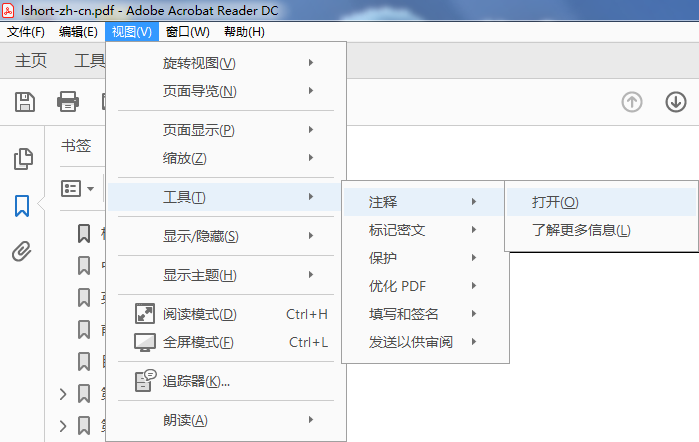
\includegraphics[width=0.85\textwidth]{02openreviewtools01}};

  % 限定坐标区域
  \begin{scope}[x={(img1.south east)},y={(img1.north west)}]
    % 绘制坐标辅助网络
    \drawgrid
    
    % 利用fit库绘制命名矩形
    \node[fit={(0.145,0.89) (0.235,0.96)}, inner sep=0pt, draw=red, thick] (view) {};
    \node[fit={(0.23,0.53) ($(0.23, 0.53) + (0.07, 0.045)$)}, inner sep=0pt, draw=red, thick] (tools) {};
    \node[fit={(0.522,0.52) ($(0.522, 0.52) + (0.05, 0.045)$)}, inner sep=0pt, draw=red, thick] (annotation) {};
    \node[fit={(0.755,0.52) ($(0.755, 0.52) + (0.075, 0.045)$)}, inner sep=0pt, draw=red, thick] (open) {};

    % 绘制箭头连线表示操作顺序(用node为连线添加标记)
    \draw[-{Stealth[scale=0.8]}, blue, thick] (view.south) to
    [out=-90, in=180] node[midway,circle,fill=blue,inner
    sep=0pt,minimum size=3pt,yellow] {\scriptsize \sffamily
      1}(tools.west); \draw[-{Stealth[scale=0.8]}, blue, thick]
    (tools.east) to [out=0, in=180]
    node[midway,circle,fill=blue,inner sep=0pt,minimum
    size=3pt,yellow] {\scriptsize \sffamily 2}(annotation.west);
    
    \draw[-{Stealth[scale=0.8]}, blue, thick] (annotation.east) to
    [out=0, in=180]node[midway,circle,fill=blue,inner
    sep=0pt,minimum size=3pt,yellow] {\scriptsize \sffamily 3}
    (open.west);
  \end{scope}  
\end{tikzpicture}

\begin{tikzpicture}
  \node[anchor=south west, inner sep=0](img1) at (0,0)
  {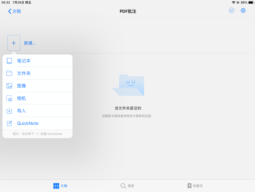
\includegraphics[width=0.45\textwidth]{04importmenu}};
  \node[anchor=south west, inner sep=0, right=0.1 of img1](img2) 
  {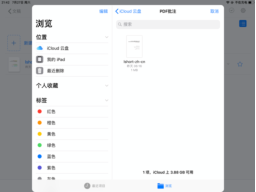
\includegraphics[width=0.45\textwidth]{05importicloud}};

  \begin{scope}[x={(img2.south east)},y={(img1.north west)}]
    % 绘制坐标辅助网络
    % \drawgrid
        
    % 利用fit库绘制命名矩形
    \node[fit={(0.23,0.92) (0.268, 0.96)}, inner sep=0pt, draw=blue, thick] (pdffold) {};        
    \node[fit={(0.008,0.731) (0.073, 0.825)}, inner sep=0pt, draw=red, thick] (new) {};
    \node[fit={(0.008,0.4) (0.055, 0.445)}, inner sep=0pt, draw=red, thick] (import) {};
    \node[fit={(0.57,0.73) (0.66, 0.77)}, inner sep=0pt, draw=red, thick] (icloud) {};
    \node[fit={(0.69,0.92) (0.78, 0.96)}, inner sep=0pt, draw=blue, thick] (icloudroot) {};
    \node[fit={(0.81,0.92) (0.85, 0.96)}, inner sep=0pt, draw=blue, thick] (icloudpdf) {};
    \node[fit={(0.74,0.62) (0.79, 0.83)}, inner sep=0pt, draw=red, thick] (pdfname) {};

    % 绘制箭头连线表示操作顺序
    \draw[-{Stealth[scale=0.8]}, blue, thick] (pdffold.west) to
    [out=180, in=90] (new.north);
        
    \draw[-{Stealth[scale=0.8]}, red, thick] (new.east) to [out=0,
    in=180] node[midway,circle,fill=black,inner sep=0pt,minimum
    size=3pt,white] {\scriptsize \sffamily 1}(import.west);
        
    \draw[-{Stealth[scale=0.8]}, red, thick] (import.east) to
    [out=0, in=180] node[midway,circle,fill=black,inner
    sep=0pt,minimum size=3pt,white] {\scriptsize \sffamily
     2}(icloud.west);
        
    \draw[-{Stealth[scale=0.8]}, red, thick] (icloud.east) to
    [out=0, in=180]node[midway,circle,fill=black,inner
    sep=0pt,minimum size=3pt,white] {\scriptsize \sffamily 3} (pdfname.west);
    
    \draw[-{Stealth[scale=0.8]}, blue, thick] (icloudroot.east) to
    [out=0, in=180] (icloudpdf.west);
        
    \draw[-{Stealth[scale=0.8]}, blue, thick] (icloudpdf.south) to
    [out=-90, in=45] (pdfname.north);        
  \end{scope}
\end{tikzpicture}

\end{document}

%%% Local Variables:
%%% mode: latex
%%% TeX-master: t
%%% End:
